\documentclass{sig-alternate}
%\documentclass{vldb}
%\documentstyle{article}
%\documentstyle[amsmath,amsthm,amssymb,twocolumn]{article}
\usepackage{times}



\usepackage{MnSymbol} 
%\usepackage{MinionPro}
%\usepackage[mathlf,textlf,minionint]{MinionPro}
%\usepackage[T1]{fontenc}
%\usepackage{textcomp}
\usepackage{multirow}
%\usepackage{times}
\usepackage{pgfplots}
\usepackage{subfigure}
%\usepackage{amsmath,amssymb}
\usepackage{graphicx,color}
%\usepackage{verbatim}
%\usepackage{framed}
%\usepackage[ruled,vlined]{algorithm2e}

\usepackage[font={scriptsize,it}]{caption}


\begin{document}



\newcommand{\agp}[1]{\textcolor{red}{Aditya: #1}}
%\newcommand{\alkis}[1]{\smallskip\noindent \textcolor{red}{\it $\Rightarrow$ Alkis: #1}}
\newcommand{\SeeDB}{{\sc SeeDB}}
\newcommand{\calQ}{\mathcal{Q}}
\newcommand{\calR}{\mathcal{R}}
\newcommand{\att}[1]{{\text{#1}}}

\newtheorem{definition}{Definition}[section]
\newtheorem{example}[definition]{Example}
\newtheorem{goal}{Goal}[section]
\renewcommand{\baselinestretch}{0.995}

%\DeclareMathOperator*{\argmax}{arg\!\max}




%\newcommand{\histvis}{\mbox{\sc HistVis}}
\newcommand{\squishlist}{
   \begin{list}{$\bullet$}
    { \setlength{\itemsep}{0pt}
      \setlength{\parsep}{2pt}
      \setlength{\topsep}{0pt}
      \setlength{\partopsep}{0pt}
      \leftmargin=25pt
\rightmargin=0pt
\labelsep=5pt
\labelwidth=10pt
\itemindent=0pt
\listparindent=0pt
\itemsep=\parsep
    }
}
\newcommand{\squishend}{\end{list}}

\newenvironment{denselist}{
    \begin{list}{\tiny{$\bullet$}}%
    {\setlength{\itemsep}{0ex} \setlength{\topsep}{0ex}
    \setlength{\parsep}{0pt} \setlength{\itemindent}{0pt}
    \setlength{\leftmargin}{0.5em}
    \setlength{\partopsep}{0pt}}}%
    {\end{list}}

\newcommand{\eat}[1]{}
\newcommand{\papertext}[1]{#1}
\newcommand{\techreport}[1]{}

\newcommand{\techreporttext}[1]{}
\newcommand{\stitle}[1]{\vspace{0.25em}\noindent\textbf{#1}}




\title{SeeDB: What's interesting about my query?\vspace{-5pt}}
%\subtitle{\vspace{-10pt}[Vision Paper]\vspace{5pt}}



%\numberofauthors{3}
%\author{
%}

\maketitle                                                                                       

%\begin{abstract}
%%!TEX root=demo-paper.tex


% Data scientists rely on visualizations to interpret the data returned by
% queries, but finding the right visualization remains a manual task that is often
% laborious. We propose a DBMS that partially automates the task of finding the
% right visualizations for a query. In a nutshell, given an input query Q, the new
% DBMS optimizer will explore not only the space of physical plans for Q, but also
% the space of possible visualizations for the results of Q. The output will
% comprise a recommendation of potentially ``interesting'' or ``useful''
% visualizations, where each visualization is coupled with a suitable query
% execution plan. We discuss the technical challenges in building this system and
% outline an agenda for future research.
% 
Data analysts operating on large volumes of data 
often rely on visualizations to interpret the results of queries. 
However, finding the right visualization for a query is 
a laborious and time-consuming task. 
We demonstrate \VizRecDB, a system that partially automates 
this task: 
given a query, \VizRecDB\ explores the space of all possible visualizations,
and automatically identifies and recommends to the analyst those visualizations
it finds to be most ``interesting'' or ``useful''.
In our demonstration, conference attendees
will see \VizRecDB\ in action for a variety of queries on multiple real-world
datasets.





%\end{abstract}

%%% This is an example first chapter.  You should put chapter/appendix that you
%% write into a separate file, and add a line \include{yourfilename} to
%% main.tex, where `yourfilename.tex' is the name of the chapter/appendix file.
%% You can process specific files by typing their names in at the 
%% \files=
%% prompt when you run the file main.tex through LaTeX.
\chapter{Introduction}
\label{sec:introduction}

This thesis presents the design and implementation of a system, \SeeDB,
for automatically generating a large number of {\it interesting visualizations}
for any given query. There are two key challenges in automatically generating
visualizations: 1) automatically determining ``interesting''-ness of a
visualization, and 2) evaluating a large number of possible visualizations
efficiently.
In this work, we present solutions to both these problems.

\section{The data analysis process}
Data analysts must sift through very large volumes of data 
to identify trends, insights, or anomalies. 
Given the scale of data, and the relative ease and 
intuitiveness of examining data visually,
analysts often use visualizations as a tool to identify
these trends, insights, and anomalies.
However, selecting the ``right'' visualization often 
remains a laborious and time-consuming task. We illustrate the data analysis
process and challenges in choosing good visualizations using a few examples.

\subsection{Example 1: Business Intelligence}
Consider a dataset containing sales records for a nation-wide
chain of stores.
Let's say the store's data analyst is interested
in examining how the newly-introduced heating device, the ``Laserwave
Oven'', has been doing over the past year.
The results of this analysis will inform business decisions
for the chain, including marketing strategies, and the introduction of a similar
``Saberwave Oven''.

The analysis workflow proceeds as follows:
(1) The analyst poses a query to select the subset of data that she is
interested in exploring.
For instance, for the example above, she may issue the query:
\noindent $${\tt \ Q \ \ = \ \ SELECT \ * \ FROM \ \  Sales \ \ WHERE \ \
Product=``Laserwave''} $$ \noindent Notice that the results for this query may
have (say) several million records each with several dozen attributes.
Thus, directly perusing the query result is simply infeasible.
(2) Next, the analyst studies various properties of the selected data by
constructing diverse views or visualizations from the data. In this particular
scenario, the analyst may want to study total sales by store, quantity in stock
by region, or average profits by month. To construct these views, the analyst
can use operations such as binning, grouping, and aggregation, and then generate
visualizations from the view. For example, to generate the view `total sales by
store', the analyst would group each sales record based on the store where the
sale took place and sum up the sale amounts per store. This operation can easily
be expressed as the familiar aggregation over group-by query:
\noindent
\begin{align*}
& \tt Q' = SELECT \ \ store,\ SUM(amount) \ \ FROM \ \  Sales \ \ WHERE \\
& \tt Product=``Laserwave" \ \ GROUP  \ \ BY \ \ store
\end{align*}
The result of the above query is a two-column table that can then be visualized
as a bar-chart. Table \ref{tab:staplerX} and Figure
\ref{fig:staplerX} respectively show an example of the results of this view and
the associated visualization.

\begin{figure}[htb]

  \centering
    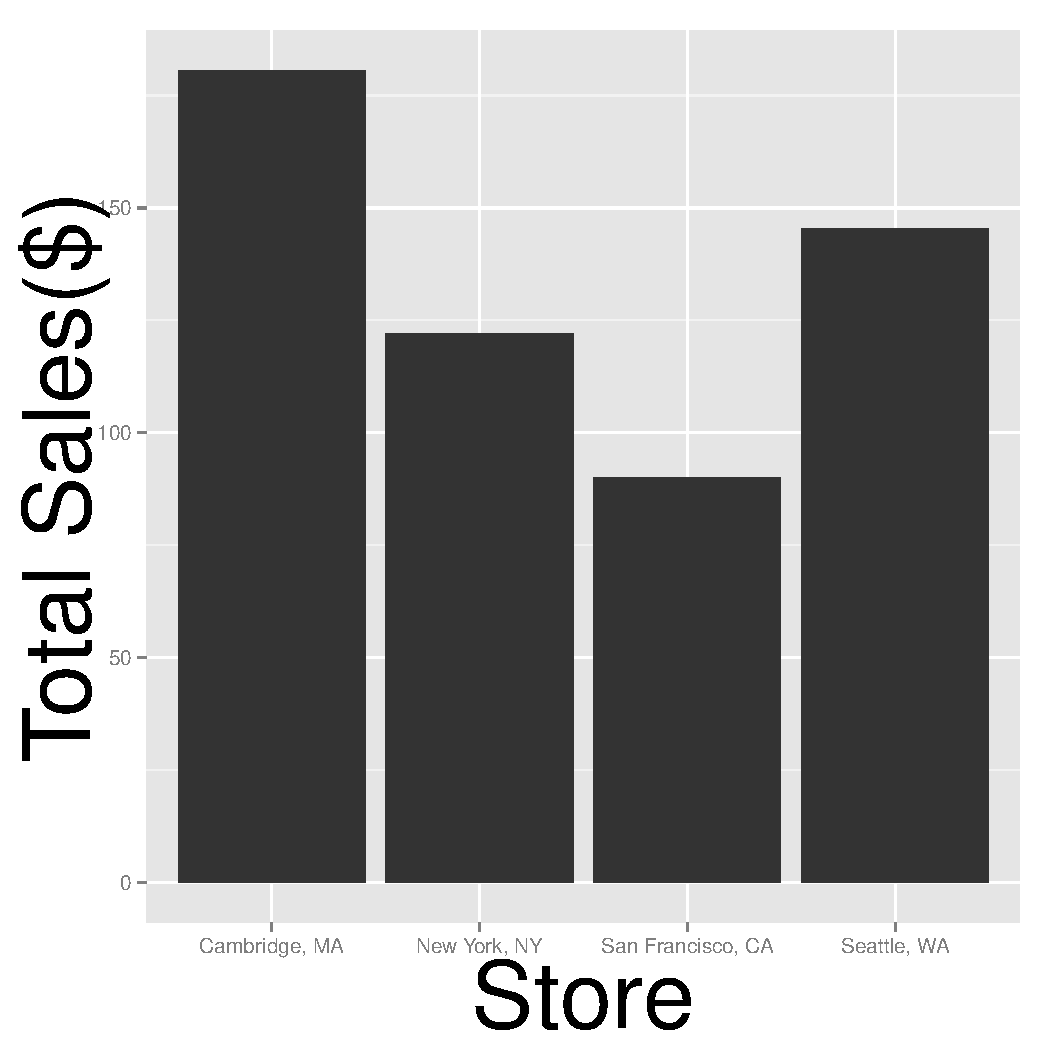
\includegraphics[width=12cm]{Images/dist1.pdf}
  \caption{Data: Total Sales by Store for Laserwave}
  \label{fig:staplerX}
\end{figure}

\begin{table}[htb]
  \centering
  \begin{tabular}{cc} \hline
  Store & Total Sales (\$) \\ \hline
  Cambridge, MA & 180.55 \\ \hline
  Seattle, WA &  145.50\\ \hline
  New York, NY & 122.00 \\ \hline
  San Francisco, CA & 90.13 \\ \hline
  \end{tabular}
  \caption{Data: Total Sales by Store for Laserwave}\label{tab:staplerX} 
\end{table}

\begin{figure}[htb]
  \centering
    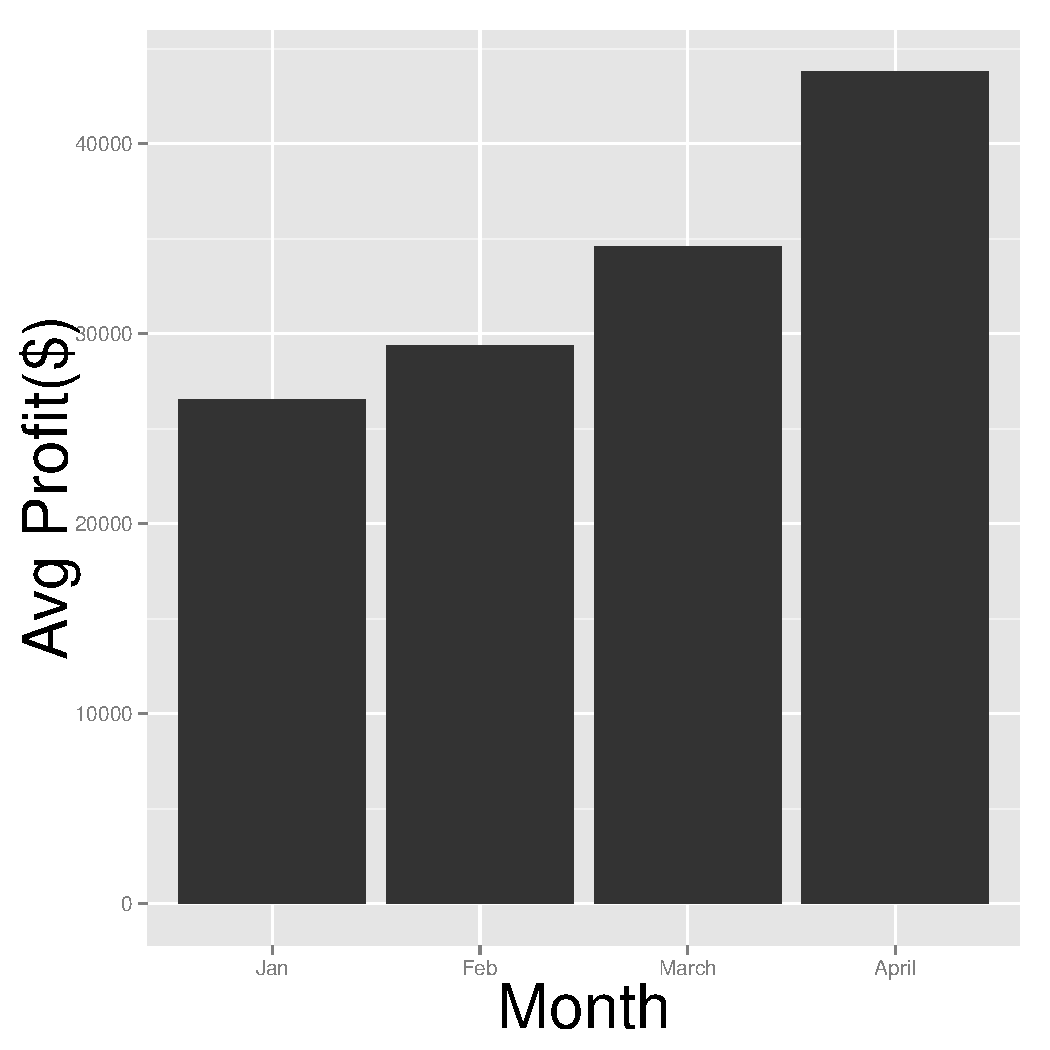
\includegraphics[width=12cm]{Images/dist2.pdf}
\caption{Scenario A: Total Sales by Store}
\label{fig:staplerX-a}
\end{figure}

\begin{figure}[htb]
  \centering
    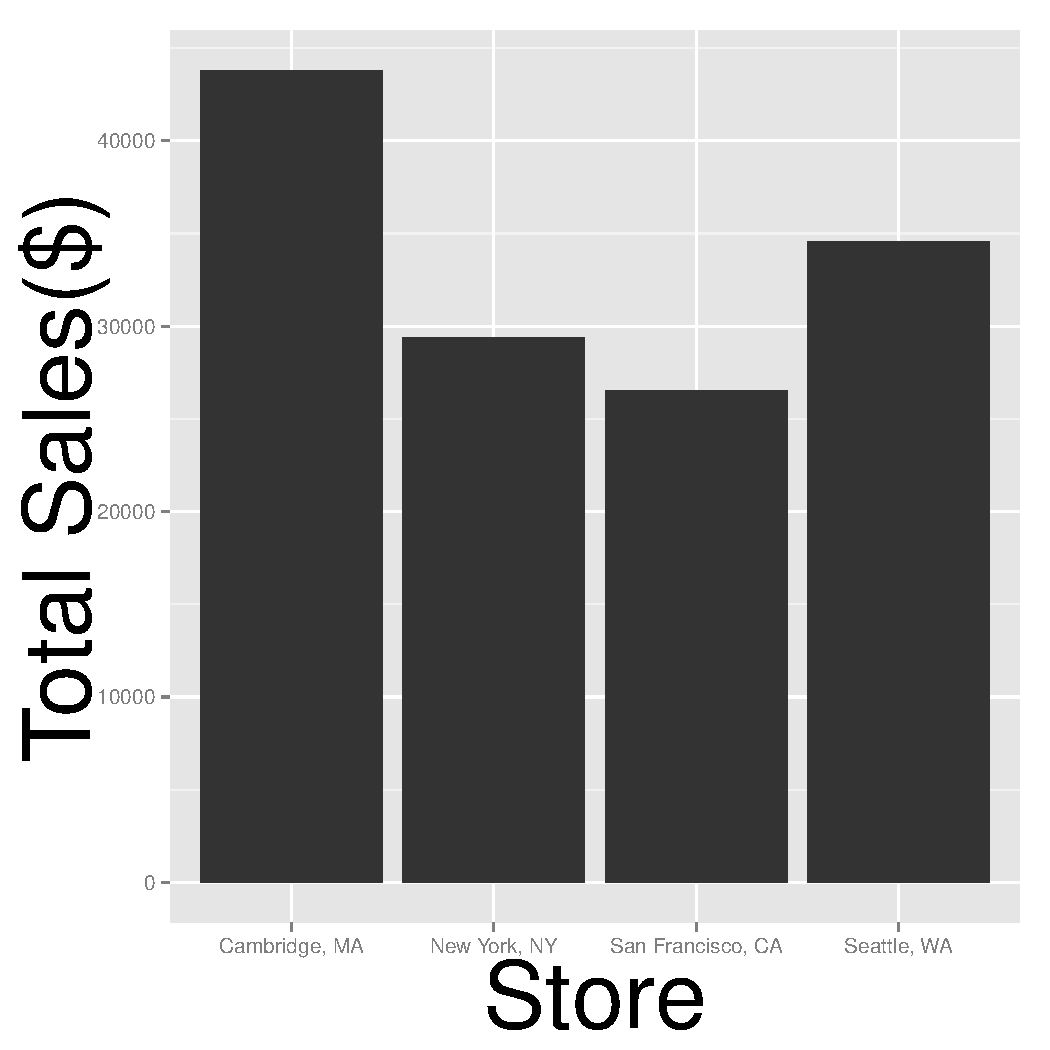
\includegraphics[width=12cm]{Images/dist3.pdf}
  \caption{Scenario B: Total Sales by Store}
  \label{fig:staplerX-b}
\end{figure}

To explore the query results from different perspectives, the analyst generates
a large number of views (and visualizations) of the form described above.
(3) The analyst then manually examines each view and decides
which ones are ``interesting''. This is a critical and time-consuming step.
Naturally, what makes a view interesting depends on the 
application semantics and the trend we are comparing against.
For instance, the view of Laserwave sales by store, as shown in Figure
\ref{fig:staplerX}, may be interesting if the overall sales of all products show
the {\it opposite} trend (e.g. Figure \ref{fig:staplerX-a}). However, the same
view may be uninteresting if the sales of all products follow a similar trend (Figure \ref{fig:staplerX-b}).
Thus, we posit that  a view is {\em potentially ``interesting'' if it shows 
a trend in the subset of data selected by the analyst
(i.e., Laserwave product-related data)
that deviates from the equivalent trend in the overall dataset}.
Of course, the analyst must decide if this deviation 
is truly an insight for this application.
(4) Once the analyst has identified interesting views, the analyst may
then either share these views with others, further interact with
the displayed views (e.g., by drilling down or rolling up), or
start afresh with a new query.


Of the four steps in the workflow described above, the 
ones that are especially repetitive and tedious are steps (2) and (3),
where the analyst generates a large number of candidate views, and examines each
of them in turn. The goal of our system, \SeeDB, is to automate these
labor-intensive steps of the workflow. Given a query $Q$ indicating the subset
of data that the analyst is interested in, \SeeDB\ automatically {\em identifies and highlights to the analyst the most
interesting views of the query results using methods based on
deviation}. Specifically, \SeeDB\ explores the space of all possible views and
measures how much each view deviates from the corresponding view on the
entire underlying dataset (e.g. Figure~\ref{fig:staplerX} vs.
Figures~\ref{fig:staplerX-a} or \ref{fig:staplerX-b}.) By generating and
scoring potential views automatically, \SeeDB\ effectively eliminates
steps (2) and (3) that the analyst currently performs. Instead, once \SeeDB\
recommends interesting views, the analyst can evaluate this small
subset of views using domain knowledge and limit further
exploration to these views.  

\subsection{Example 2: Medical Data}
Next, let us examine a use case in a completely different problem domain that
also involves analyses similar to Example 1, and therefore, can benefit from the
automatic construction of interesting views of a user query.

Consider a medical researcher studying the cost of care for cancer
patients\footnote{Real use scenario at an area hospital}. The goal of the study
is to identify patients whose cost of care is significantly greater than
average and try to explain the high cost of care. Potential reasons for
high cost include treatments for late-stage cancers, old age of the
population, longer survival time (chemotherapy for a longer duration), type of
treatment etc.
Note that the goal is {\it not} to build a predictive model for cost; rather, it
is to perform exploratory analysis to explain {\it why} certain patients have
high cost of care.
As a first pass, assume that the researcher identifies high cost patients as those with
cost that is greater than two standard deviations away from the average
cost. This can be expressed via the following SQL query, assuming a table of
patients with their treatment costs and other treatment-related information.
\begin{align*}
& \tt Q2\ = SELECT \ \ *\ FROM \ \ Patients \ \ where\ cost - \\
  \ \ & \tt (SELECT\ AVG(cost)\ FROM\ Patients)\ >\\
  \ \ & \tt 2\ *\ (SELECT\ STDDEV(cost)\ FROM\ Patients)
\end{align*}

Once these patients have been identified, the researcher can begin to analyze
the data to find potential reasons for their high cost of care (This is similar
to Step 1 in Example 1).
One technique to find potential reasons for high cost is to compare the
high-cost population of patients to the remaining set of patients (called
``low-cost'' population).
Similar to Example 1 above, we posit that the {\it characteristics that
explain high cost are precisely those characteristics that are different between
the high-cost and low-cost population}. 
For instance, if the majority of
high-cost patients were those with late-stage disease (sicker patients) while
the low-cost patients were not, the researcher could reason that the sicker
patients needed more medications or procedures, leading
to higher cost overall. 
Note that this analysis is similar to Example 1 where we
compared the ``total sales by year'' for $Laserwave$ $oven$ vs. all store
products.
In this setup, we want to compare the ``total patients by disease stage'' for
high-cost patients vs. low-cost patients. The only change in the problem
formulation is that we are now comparing views of query Q2 against views of the
remaining table, instead of views over the entire table. The rest of the
framework remains unchanged. Therefore, \SeeDB\ can be used to automatically
construct a large number of views of the high-cost population, compare
each view to the corresponding view over the low-cost population, and
identify views showing the highest difference between the two populations. These
views identify potential causes for high cost. Once the researcher has identified views of interest, he or she
can follow up with more complex analyses like statistical significance testing or machine
learning.

\subsection{Example 3: Product Analysis}

Consider a company like Facebook\footnote{www.facebook.com} that continuously
deploys changes to its website and mobile apps, and tracks user interaction
through detailed logging. Product specialists at Facebook use these logs to
study how different Facebook users respond to changes to the web or mobile
experience \cite{DBLP:conf/vldb/AbrahamABB13}. Each user can be characterized by a large number
of features such as location, age, device used, number of friends etc.
For each user, the logs note the actions taken on the website or app such
as likes, shares, comments, page visits etc. For example, in order to study
the user response to an update to the mobile app, the specialist compares user
interaction metrics for a large number of mobile users before and after the
update (usually a week on week comparison). The goal is to find patterns in the
interaction metrics based on different user characteristics. Therefore, if it
appears that the average number of app visits on the iOS app have reduced
signficantly following the update, it would indicate a problem with the iOS app.

In terms of the \SeeDB\ framework, log data from the week following the app
update constitutes the query results we seek to analyze and the log data from
the prior week comprises the comparison dataset. As in Examples 1 and 2, the
analysis process requires the specialist to create diverse views of the query
results, compare views to equivalent views on the comparison dataset, and
pick the views showing the highest difference. 
\SeeDB\ can therefore be used to automate this process and surface only the most
interesting views.

\subsection{\SeeDB}
This thesis describes a prototype of the \SeeDB\ system that finds interesting
visualizations of query results. 
Given a query $Q$ indicating the subset of data that the analyst is interested in, \SeeDB\ automatically {\em identifies and highlights to the
analyst the most interesting views of the query results using methods based on
deviation}. 
Our prototype is based on
\cite{DBLP:conf/vldb/Parameswaran2013} which describes the vision for \SeeDB.

To efficiently and accurately identify interesting views of any given query, we
are faced with the following challenges:
\begin{itemize}
  \item We must determine metrics that accurately measure the ``deviation'' of a
view with respect to the equivalent view on the entire database (e.g.,
Figure~\ref{fig:staplerX} vs.~\ref{fig:staplerX-a}), while simultaneouly
ensuring that \SeeDB\ is not tied to any particular metric(s)
\item We must
intelligently explore the space of candidate views. Since the number of
candidate views (or visualizations) increases as the square of the number of
attributes in a table (we will demonstrate this in subsequent sections),
generating and evaluating all views, even for a moderately sized dataset (e.g.
1M rows, 100 attributes), can be prohibitively expensive
\item While executing
queries corresponding to different views, we must share computation as much as
possible. For example, we can compute multiple views and measure their deviation
all together in one query. Independent execution, on the other hand, will be
expensive and wasteful
\item Since analysis must happen in real-time, we must trade-off accuracy of
visualizations or estimation of ``interestingness'' for reduced latency.
\end{itemize}

Contributions of the work described in this thesis are:
\begin{itemize}
  \item We implement the \SeeDB\ system based on \cite{DBLP:conf/vldb/Parameswaran2013} to
  automatically find interesting views of queries (Chapter
  \ref{sec:system_architecture}).
  \item We propose and implement a number of optimizations to
  efficiently perform the search for interesting views and share
  computation between multiple views simultaneously (Chapter
  \ref{sec:optimizations}).
  \item We evaluate the performance of our optimizations on a range of datasets
  and demonstrate the resulting 100x speedup (Chapter
  \ref{sec:experiments}).
  \item We model the performance of \SeeDB\ in terms of various parameters of
  \SeeDB\ and the underlying database, and use this model to identify optimal
  parameter settings for \SeeDB\ (Chapter \ref{sec:model}).
  %\item We present and evaluate different metrics for measuring deviation
  %\item ?? We study the usefulness of a tool like \SeeDB\ in finding
  %interesting visualizations of a dataset
\end{itemize}



% of Step 1), we demonstrate that we can automatically explore various views of
% that data, evaluate each one for ``interesting''-ness and only surface the most
% promising views to the analyst. 



% In this demo, we demonstrate a system called \SeeDB\
% \cite{DBLP:conf/vldb/Parameswaran2013} that automates the labor-intensive parts
% of the aforementioned data analysis process by automatically identifying and
% producing high-quality views for any input query. Specifically, given a query
% $Q$ posed by the user, \SeeDB\ explores all possible views of $Q$, determines
% the ``interesting''-ness of each of the views based on deviation and returns to
% the user the set of views that it deems the most interesting. The user can then
% limit his analysis to this high-quality set of views.

% In the process of automatically producing an interesting set of views for any
% query, \SeeDB\ must address a few challenges: (a) the size of the space of
% potential views increases as the square of the number of attributes in a table,
% and even for a moderately sized table (e.g. 1M rows, 100 attributes) generating
% all views is prohibitively expensive; as a result, \SeeDB\ must intelligently
% explore this space; (b) computing each view and its utility independently is
% expensive and wasteful, and hence \SeeDB\ must share computation between
% queries; and (c) since visual analysis must happen in real-time, \SeeDB\ must
% tradeoff accuracy of views for reduced latency. In Section
% \ref{sec:system_architecture}, we describe how \SeeDB\ addresses these
% challenges.


% Consider a medical researcher studying the cost of care for cancer patients. Her
% research involves the analysis of a set of 1M electronic medical records (EMRs).
% To analyze this data, the researcher identifies patients that cost
% significantly more than the average: specifically, she selects patients whose
% cost of care is greater than the average cost by two standard deviations. In
% terms of SQL, she runs the following query: \\

% \noindent 
% \begin{small}
% \begin{verbatim}
% Q = SELECT * FROM Patients where total_cost - 
% (SELECT AVG(total_cost) from Patients) as avg_cost
% > 2 * (SELECT STDDEV(total_cost) from Patients);
% \end{verbatim}
% \end{small}

% Once she has identified these patients, she must study various aspects of their
% care to determine the reason why the patients have large cost of care. For
% instance, she may study length of treatment, survival rate, severity of disease
% etc. For each of these parameters, she is interested in determining how the
% group of patients with high cost of care are different from the overall group of
% patients. As a result, she may construct various views of the data that
% compare various metrics between the high cost patients and the overall patient
% population. For instance, she may compare the distribution of length of
% treatment for the two populations, the average severity of the disease
% etc. Since there are a large number of metrics that may be responsible for high
% cost of care, the analyst must construct, visualize and examine a large number
% of views to identify interesting trends. For more than 5 metrics, this process
% quickly becomes tedious and time-consuming. We can significantly simplify and
% speed up the analysis process if we can automate the creation and evaluation of
% views.


% \begin{figure}
% \vspace{-10pt}
% \CenterFloatBoxes
% \begin{floatrow}
% \ttabbox{%
%   \small
%   \begin{tabular}{cc} \hline
%   Store & Total Sales (\$) \\ \hline
%   Cambridge, MA & 180.55 \\ \hline
%   Seattle, WA &  145.50\\ \hline
%   New York, NY & 122.00 \\ \hline
%   San Francisco, CA & 90.13 \\ \hline
%   \end{tabular}
% }{%
%   \caption{Data: Total Sales by Store for Laserwave}\label{tab:staplerX}%
% }
% \killfloatstyle
% \ffigbox{%
%   \hbox{\resizebox{2cm}{2cm}{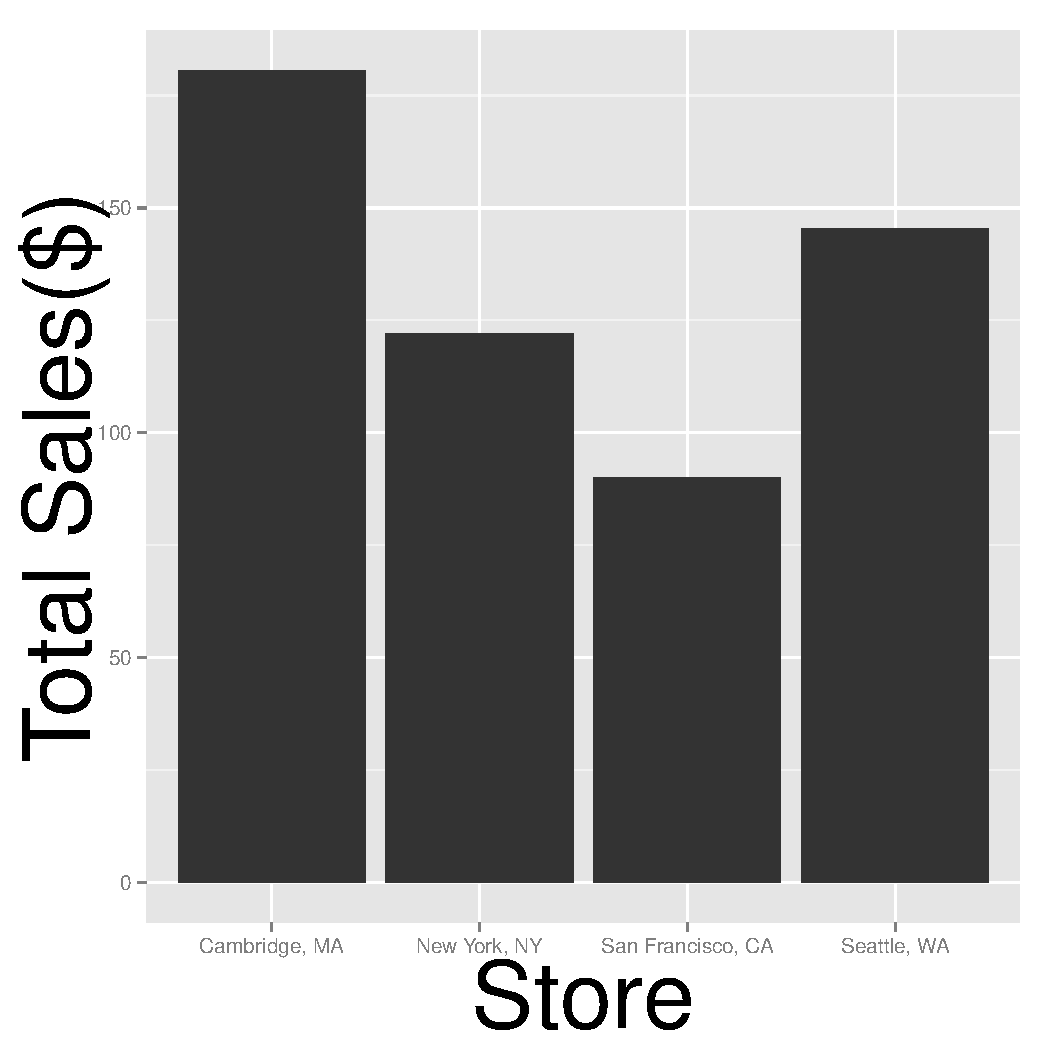
\includegraphics{Images/dist1.pdf}}}
%   
% }{%
%   \caption{Visualization: Total \\ Sales by Store for
%   Laserwave}
%   \label{fig:staplerX}%
% }
% \end{floatrow}
% \end{figure} 
%  
% \begin{figure}
% \CenterFloatBoxes
% \begin{floatrow}
% \centering
% \ffigbox{%
%   \hbox{\resizebox{2cm}{2cm}{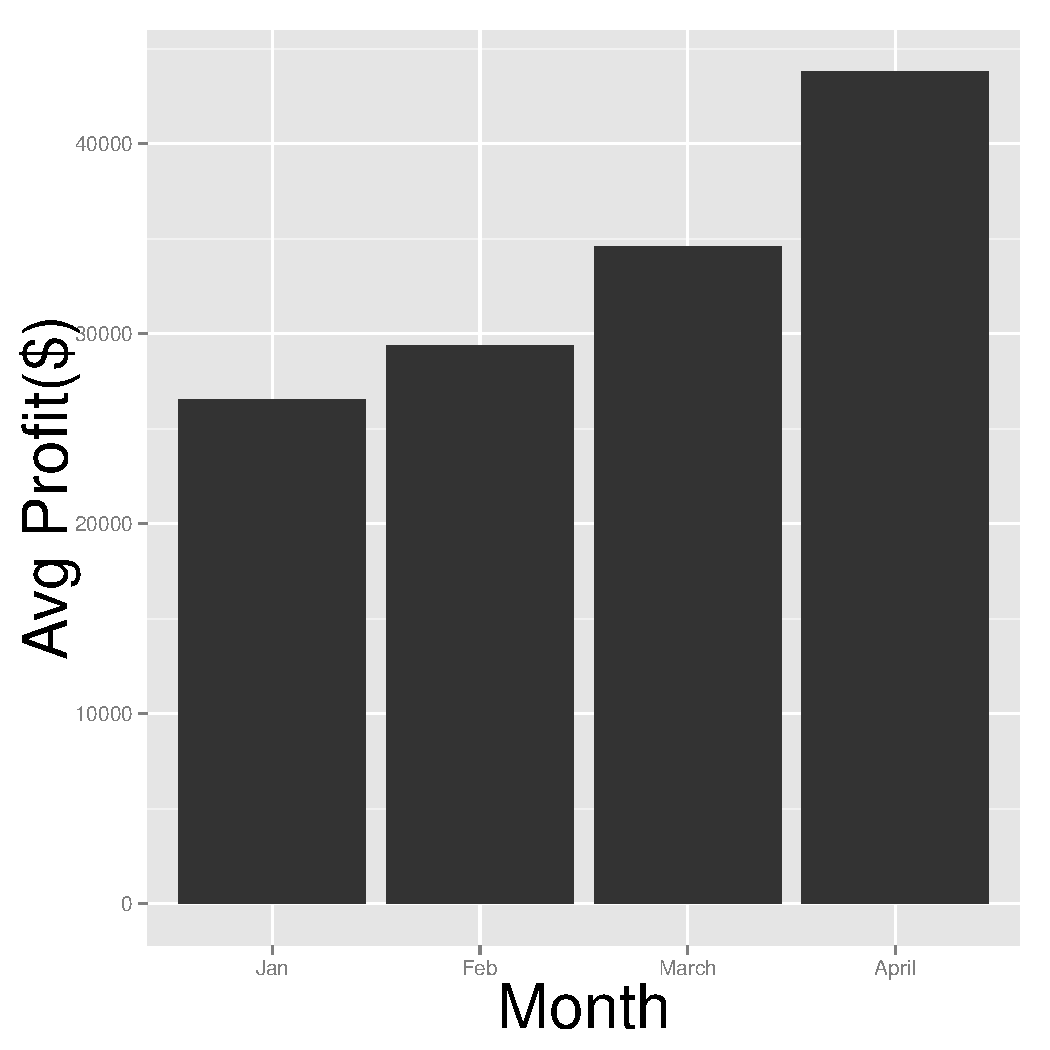
\includegraphics{Images/dist2.pdf}}}
% 
% }{ \caption{Scenario A: Total Sales by Store}\label{fig:staplerX-a}%
% }
% \killfloatstyle
% \ffigbox{%
%   \hbox{\resizebox{2cm}{2cm}{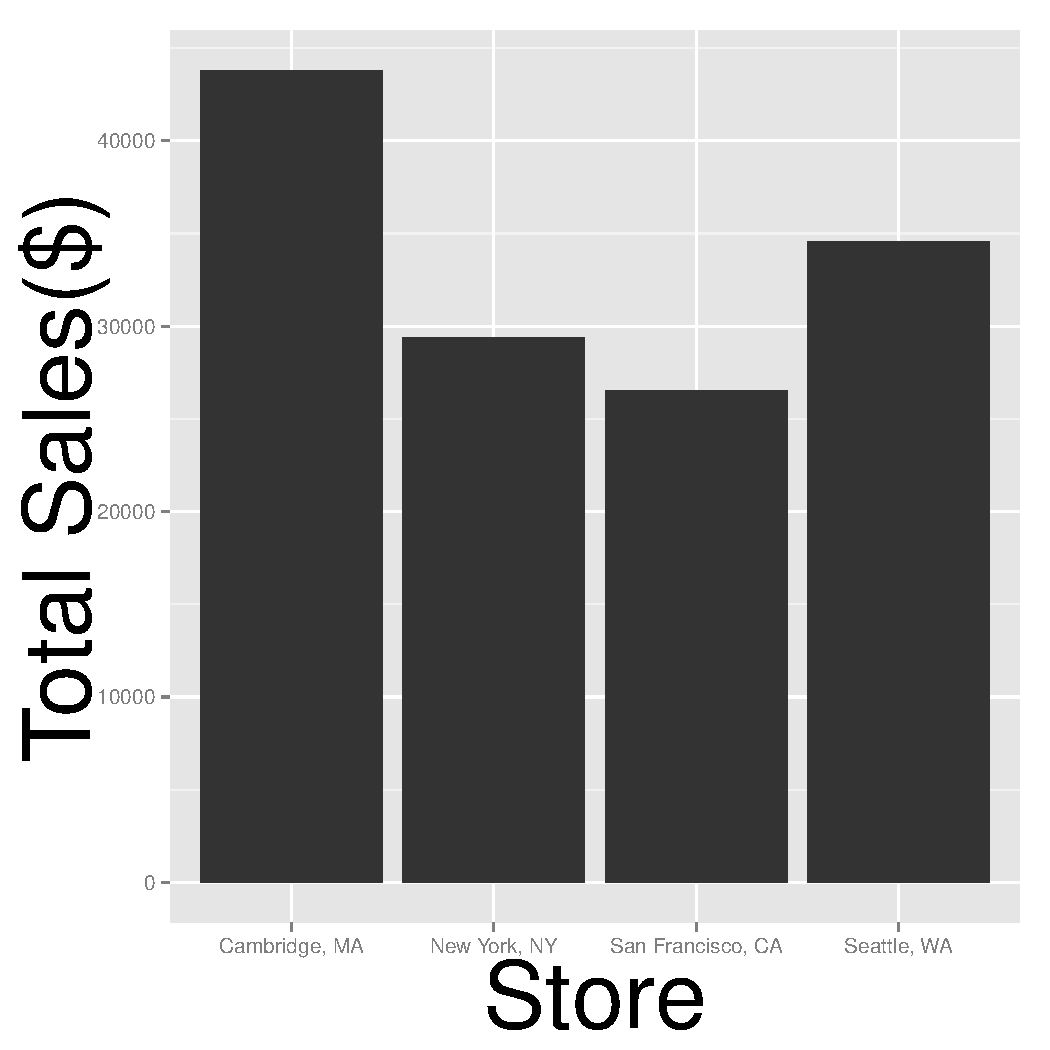
\includegraphics{Images/dist3.pdf}}} 
% 
%   }{\caption{Scenario B: Total Sales by Store}
%   \label{fig:staplerX-b}%
%   }
% \end{floatrow}
% \vspace{-12pt}
% \end{figure}


% Since \SeeDB\ must rank views based on utility, accurately measuring 
% utility is cruicial. \SeeDB\ is based on the principle
% that it is the {\bf deviations from expected behavior that make a view
% interesting}. For instance, in the above example, the researcher would be
% interested in the fact that high-cost patients actually visit a specific set of
% doctors compared to the entire patient population. Similarly, the researcher
% would be interested in knowing that the high-cost patients have longer hospital
% stays compared to the rest of the population. Thus, given a query, interesting
% trends are those that differ significantly between the query and the underlying
% dataset. \SeeDB\ therefore assigns higher utility to views that show divergent
% trends. (Since it may be more appropriate to compare the high-cost patients with
% other patients having the same disease but lower cost, so \SeeDB\ allows the
% user to specify what dataset to compare with).


% \noindent There are several technical challenges that need to be addressed:
% 
% \begin{denselist}
% 
% \item For a given query, $n$, the total number of discriminating views, (even if
% we restrict ourselves to views that append a group-by and an aggregation) is
% likely to be very large to explore exhaustively and precisely. Generating each
% of $R_1(Q(D)),$  $\ldots,$ $R_n(Q(D))$, scoring them on utility, and then
% picking the best one is certainly not feasible for most databases. Thus, we need
% mechanisms to prune the space of views and compute their utility approximately.
% 
% \item Generating and scoring the discriminating views $R_i(Q(D))$ one-by-one may
% miss interesting optimization opportunities: First, we may share computation
% between discriminating views.  For example, the results of two views with
% different aggregates but the same group-by may be computed together in one
% query, followed by projecting out to reveal the two individual views.  Second,
% by evaluating the discriminating views in a deliberate order, we may be able to
% prune views with low utility (without evaluation) that are definitely not going
% to be recommended to the analyst.
% 
% \item Since visualizations tend to convey approximate information, e.g., a trend
% in a line plot may be more important than knowing the exact coordinates of each
% point, we can introduce approximations as part of \SeeDB.  Thus, the utility of
% a discriminating view may be computed approximately but efficiently, and the
% recommended discriminating views can be populated with approximate results,
% based on synopses of the base data or of the query result, that can be generated
% much more efficiently.
% 
% \end{denselist}

\section{System architecure}
\label{sec:system_architecture}

In this section, we present the architecture of \SeeDB\ starting with an
overview, followed by a detailed discussion of the various modules in \SeeDB.

\subsection{\SeeDB\ architecture overiew}
\label{subsec:overview}

Our prototype of \SeeDB\ is designed as a layer on top of a relational database
system.
While optimization opportunities are restricted by virtue of being outside the
database, our design permits \SeeDB\ to be used in conjunction with a variety of
existing database systems. \SeeDB\ is comprised of two main parts: the \SeeDB\
front end and the \SeeDB\ backend. The front end is a ``thin client'' that
is only used to issue queries to \SeeDB\ and view results. The backend in
contrast performs all the computation required to generate and select views. Figure \ref{fig:sys-arch}
shows the architecture of our system.

\begin{figure}[htb]
\centerline{
\hbox{\resizebox{9cm}{!}{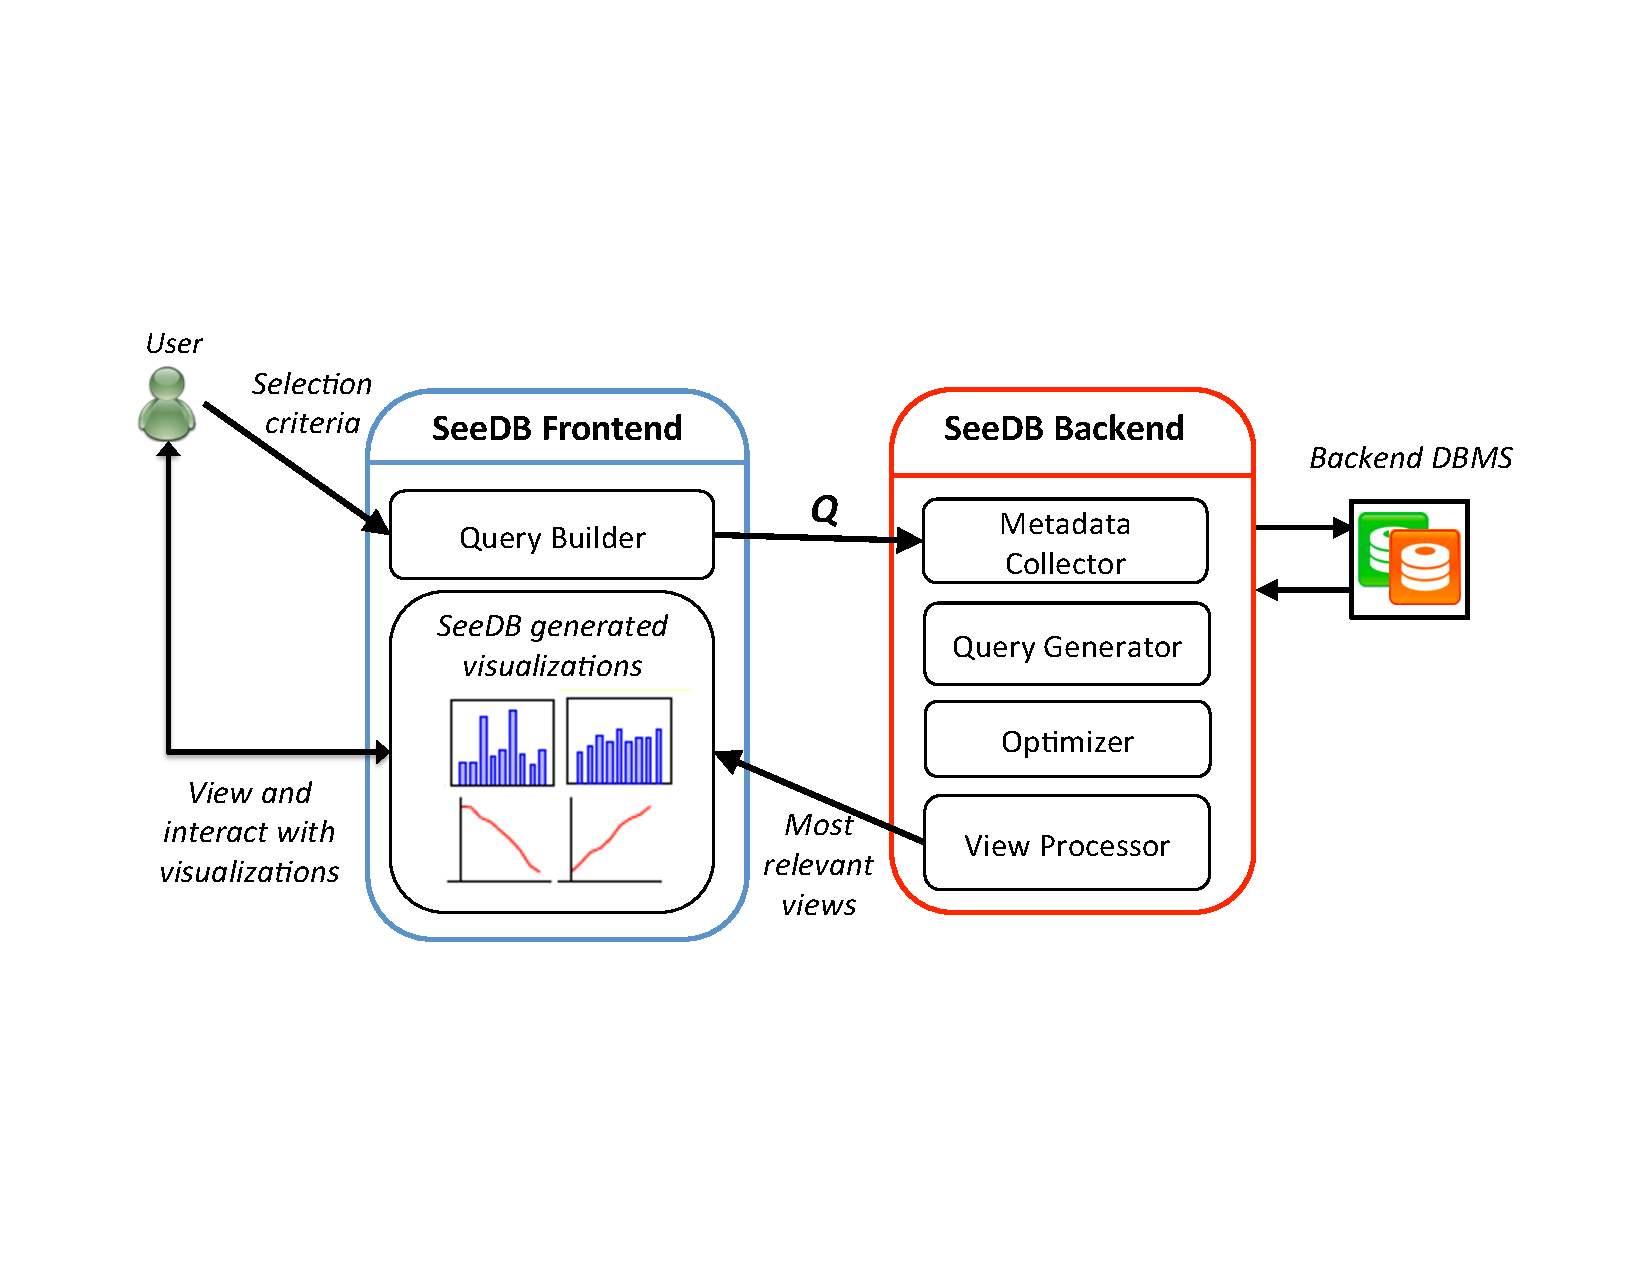
\includegraphics[trim=10mm 50mm 10mm 50mm,
clip=true]{Images/seedb-architecture.pdf}}}}
\caption{SeeDB Architecture}
\label{fig:sys-arch}
\end{figure} 

An analyst uses the front end to issue queries to \SeeDB. We provide three
mechanisms for the analyst to issue queries: raw SQL, an intuitive
query-builder, and a set of pre-formulated queries for common operations on a
dataset (we discuss query input further in Section \ref{subsec:seedb_frontend}).
Once the analyst issues a query via the \SeeDB\ front end, the backend
takes over.
First, the Metadata Collector module queries metadata tables (a combination of
database-provided and \SeeDB\ specific tables) for information such as table
sizes, column types, data distribution, and table access patterns.
The resulting metadata along with the analyst's query is then passed to the
Query Generator module. The purpose of the Query Generator is two-fold:
first, it uses the metadata obtained in the previous step to prune the space of
candidate views to the most promising ones; and second, it generates target and
comparison views for each view that has not been pruned.
The SQL queries corresponding to the target and comparison views are then passed
to the Optimizer module. We refer to these queries collectively as {\it view
queries}.
The Optimizer module is responsible for determining the best way to combine
view queries intelligently so that the total execution time is
minimized. 
(We discuss the optimizations performed by the Query Generator and
Optimizer modules further in Section \ref{subsec:seedb_backend}.) Once the
Optimizer module has generated the optimized queries, \SeeDB\ sends the
queries to the underlying database system for execution. The results returned by
the DBMS are then processed by the View Processor module. This module processes
results of the optimized queries in a streaming fashion and produces results for
individual views. Results of individual views are then normalized as discussed
in Section~\ref{sec:problem_statement} and the utility of each view is computed.
Finally \SeeDB\ selects the top $k$ views with the highest utility and returns them to the
\SeeDB\ front end. The \SeeDB\ frontend creates visualizations for each
view and displays the visualizations to the analyst.

We now discuss the major \SeeDB\ modules in detail.

\subsection{SeeDB Frontend}
\label{subsec:seedb_frontend}

The \SeeDB\ frontend, designed as a thin client, performs two main functions: it
allows the analyst to issue a query to \SeeDB, and it visualizes the results (views) produced by the \SeeDB\
backend.
To provide the analyst maximum flexibility in issuing queries, \SeeDB\
provides the analyst with three
mechanisms for specifying an input query: 
(a) writing raw SQL, (b) using a query builder that allows analysts
unfamiliar with SQL to formulate queries through a form-based interface, and (c)
using pre-defined query templates which encode commonly performed operations,
e.g., selecting outliers in a particular column. We find that pre-defined query
templates are particularly useful since analysts are often interested in
anomalous data points.

Once the analyst issues a query via the \SeeDB\ frontend, the \SeeDB\ backend
evaluates various views and sends the most interesting ones back to the
frontend.
For each view returned by the backend, the \SeeDB\ frontend determines the best
way to visualize the view depending on parameters such as the data
type (e.g. ordinal, numeric), number of distinct values and semantics (e.g.
geography vs.
time series).
The resulting set of visualizations is displayed to the analyst who can easily
examine these ``most interesting'' views at a glance, explore specific views in detail and
view metadata for each view (e.g. size of result, sample data, value with
maximum change and other statistics). 
The analyst can also slice-and-dice views further by performing drill-downs on
the relevant attributes in the view. 
Figure~\ref{} shows a screenshot of the \SeeDB\ frontend in action.
%This action automatically
%modifies the selection query and displays views for the subset of data
% selected. The user can of course revert back to the original views and continue exploring the data.

\subsection{SeeDB Backend}
\label{subsec:seedb_backend}

As discussed in Section \ref{subsec:overview}, \SeeDB\ is implemented using a
light-weight frontend described in the previous section and a backend that
performs all the computations for generating and selecting views. Furthermore,
as shown in Figure~\ref{fig:sys-arch}, the \SeeDB\ backend is composed of four
modules that are respectively responsible for collecting metadata (Metadata Collector), pruning
the view space and generating view queries (Query Generator), optimizing view
queries (Optimizer), and processing query results to identify the top-$k$
interesting views (View Processor). In this section, we will discuss the various
techniques underlying \SeeDB. To achieve its goal of finding the most
interesting views accurately and efficiently, \SeeDB\ must not only accurately
estimate the accuracy of a large number of views but also design ways in which
the total processing time will be minimized.
We first describe the basic \SeeDB\ framework and then briefly discuss our optimizations.

% One of the chief challenges in \SeeDB\ is producing the most interesting views
% of the query result in the least possible time. For achieve the above
% performance goal, \SeeDB\ must perform optimizations at two stages: first, using
% prior knowledge such as statistics to prune out uninteresting views without examining table data; and second, minimizing the
% execution time for queries that are issued to the database. 

\subsubsection{Basic Framework}
\label{subsubsec:basic_framework}

Given a user query $Q$, the basic technique used in \SeeDB\ computes all
possible views obtained by adding a single aggregate and a single group-by
clause to $Q$. Target and comparison views corresponding to each view are then
computed and each view query is executed independently on the DBMS. The query
results for each view are normalized to compute the target and comparison view
probability distributions. The utility of a given view is computed as the
distance between these two distributions (Section \ref{sec:problem_statement}).
Finally, the top-$k$ views with the largest utility are chosen. 

The basic approach is clearly inefficient
since it examines each possible view and executes each view query independently;
we next discuss how our optimizations fix some of these problems.

\subsubsection{View Space Pruning}
\label{subsubsec:view_space_pruning}

Most views possible for any query $Q$ have low utility since the target view
distribution is very similar to the comparison view distribution. 
As a result,
\SeeDB\ aggressively prunes view queries that are unlikely to have high
utility. 
This pruning is based on metadata about the table including data
distributions and access patterns.
We leverage table metadata in several ways, some of which are listed below:
\begin{denselist}
\item {\it Variance-based pruning}: Dimension attributes with low variance are
likely to produce views having low utility (e.g. consider the extreme case where
an attribute only takes a single value); as a result, \SeeDB\ prunes views
containing grouping attributes with low variance.
\item {\it Correlated columns}: If two dimension attributes $a_i$ and $a_j$ have
a high degree of correlation (e.g. full name of airport and abbreviated name of
airport), the views generated by grouping the table on $a_i$ and $a_j$ will be
very similar (and have almost equal utility). We can therefore generate and
evaluate a single view representing both $a_i$ and $a_j$. \SeeDB\ clusters
attributes based on correlation and evaluates a single representative view per
cluster.
\item {\it Access Frequency Pruning}: In tables with a large number of
attributes, only a small subset of attributes are relevant to the analyst and
are frequently accessed for data analysis. \SeeDB\ tracks access patterns
for each table to identify the most frequently accessed columns and combinations of
columns. While creating views, \SeeDB\ uses this information to prune attributes
that are rarely accessed and are thus likely to be unimportant.
\end{denselist}

\subsubsection{View Query Optimizations}
\label{subsubsec:optimizations}

The second set of optimizations used by \SeeDB\ minimizes the execution time for
view queries that haven't been pruned using the techniques described above.
Since view queries tend to be very similar (they differ in the aggregation
attribute, grouping attribute or subset of data queried) \SeeDB\ uses multiple
techniques to intelligently combine view queries.
The ultimate goal is to minimize scans of the underlying dataset by sharing as
many table scans as possible. Our optimization strategies include:

\begin{denselist}
  \item {\it Combine target and comparison view query}: Since the target view
  and comparison views only differ in the subset of data that the query is
  executed on, we can easily rewrite these two view queries as one.
  This simple optimization halves the time required to compute the results for
  a single view.
  \item {\it Combine Multiple Aggregates}: A large number of view
  queries have the same group-by attribute but different aggregation attributes.
  Therefore, \SeeDB\ combines all view queries with the same group-by attribute
  into a single query. This rewriting provides a speed up linear in the
  number of aggregate attributes.
  \item {\it Combine Multiple Group-bys}: 
  Because \SeeDB\ computes a large number of group-bys, one significant
  optimization is to combine queries with different
  group-by attributes into a single query with multiple group-bys attributes.
  For instance, consider views $(a_1$, $m_1$, $f_1)$, $(a_2$, $m_1$, $f_1)$
  \ldots $(a_n$, $m_1$, $f_1)$. Instead of executing queries for each view
  independently, we can combine the $n$ views into a single view represented by
  $(\{a_1, a_2\ldots a_n\}$, $m_1$, $f_1)$. 
  While this optimization has the potential to significantly reduce query
  execution time, the number of views that can potentially be combined depends
  closely on the correlation between values of the grouping attributes and system parameters like the
  working memory. Given a set of candidate views, we model the problem of
  finding the optimal combinations of views as a variant of bin-packing and
  apply ILP techniques to obtain the best solution (We discuss our model and
  algorithm in our full paper~\ref{}).
%   A variation of this approach also implemented
%   on \SeeDB\ is to send the results of the multiple group-by query to the front
%   end and ask the \SeeDB\ frontend to compute utility and select views. The
%   advantage of this approach is that it allows for more efficient interactive
%   exploration of the views.
  \item {\it Sampling}: For datasets of large size, the optimization that can
  have the most impact on latency is reducing the data size by
  constructing sample and running all queries against the sample. As
  expected, the sampling technique and size of the sample significantly affects
  the accuracy of the generated views. 
  \item {\it Paralle Query Execution}: The final optimization employed by
  \SeeDB\ is to take advantage of parallel processing in order to reduce total
  latency. We observe that as the number of queries executed in parallel
  increases, the total execution time does down but this comes at the cost of
  increased per query execution time.
\end{denselist}

%\begin{figure}[htb]
%\centerline{
%\hbox{\resizebox{9cm}{!}{\includegraphics[trim=10mm 50mm 10mm 50mm,
%clip=true]{Images/seedb-frontend.pdf}}}}
%\caption{SeeDB Frontend}
%\label{fig:frontend}
%\end{figure} 



%!TEX root = demo-paper.tex
\vspace{-2mm}
\section{Demo Walkthrough}
\label{sec:demo-walkthrough}
 
We propose to demonstrate the functionality of \SeeDB\ through hands-on
interaction with a variety of datasets. Our goals are two fold: (1) demonstrate
the utility of \SeeDB\ in surfacing interesting trends for a query
and (2) demonstrate that we can return high quality views efficiently for
a range of datasets. We will use four different datasets in our demonstration:

\begin{denselist}
  \item {\bf Store Orders dataset}~\cite{superstore}: This dataset is
    often used by Tableau~\cite{tableau} as a canonical dataset for
    business intelligence applications. It consists of information
    about orders placed in a store including products, prices, ship
    dates, geographical information, and profits. Interesting trends in
    this dataset have been very well studied, and attendees will use
    \SeeDB\ to quickly re-identify these trends. 
    %This dataset will also
    %enable us to demonstrate how \SeeDB can correctly deal with
    %numeric, categorical, and geographic data.
  \item {\bf Election Contribution dataset}~\cite{election_data}: This
  is an example of a dataset typically analyzed by
    non-expert data analysts like journalists or historians. With this
    dataset, we demonstrate how non-experts can use \SeeDB\ to quickly
    arrive at interesting visualizations.
  \item {\bf Medical dataset~\cite{mimic}:} This real-world dataset exemplifies
  a dataset that a clinical researcher might use. The schema of the dataset is
  significantly complex and it is of larger size.  
    \item {\bf Synthetic data:} We provide a set of synthetic datasets with
    varying sizes, number of attributes, and data distributions to help
    attendees evaluate \SeeDB\ performance on diverse datasets.
\end{denselist}

\stitle {Scenario 1: Demonstrating Utility.} Attendees are provided with three
diverse, real-world datasets to explore using \SeeDB. For each dataset,
attendees can issue ad-hoc or pre-formulated queries to \SeeDB. \SeeDB\ will
then intelligently explore the view space and optimize query execution to return the
most interesting visualizations with low latency. Attendees can examine the
returned queries visually, via the associated view metadata, and via
drill-downs. To aid the evaluation of visualizations, the demo system will show
the user a set of ``bad'' views (views with low utility) that were not selected
by \SeeDB.
Similarly, we provide pre-selected queries (and
previously known information about their results) to allow attendees to
confirm that \SeeDB\ does indeed reproduce known information about these
queries. Attendees will also have the ability to experiment with a
variety of distance metrics for computing utility and observe the effects on the
resulting views.

% \stitle{Demonstrating Utility:} To show the utility of \SeeDB\ in a real-world
% scenario, we will provide conference attendees three diverse datasets that they
% can explore and interact with. Attendees can pose ad-hoc or pre-selected queries
% on various datasets and evaluate the visualizations returned. The
% evaluation is based on whether the visualizations surface ``interesting''
% aspects of the queried data and whether the right visualizations have been
% selected. To aid the evaluation of visualizations, the demo version of \SeeDB\
% will have the option of showing ``bad'' visualizations too, i.e. visualizations
% that were predicted to have low utility.  The attendees will also have the option of
% trying various utility metrics as described in Section
% \ref{sec:problem_statement}. The demo datasets will include:

\stitle{Scenario 2: Demonstrating Performance and Optimizations.} This scenario
will use an enhanced user interface and synthetic datasets mentioned above.
Attendees will be able to easily experiment with a range of datasets and input
queries by tuning various ``knobs'' such as data size, number of attributes, and
data distribution. In addition, attendees will also be able to select the
optimizations that \SeeDB\ applies and observe the effect on response times and
accuracy.

Thus, through our demonstration of \SeeDB\, we seek to illustrate that (a) it is
possible to automate labor-intensive parts of data analysis, (b) aggregate
and grouping-based views are a powerful means to identify interesting trends
in data, and (c) the right set of optimizations can enable real-time data
analysis of large datasets.

\eat{
We propose to demonstrate the functionality of the SeeDB system by means of
analyzing three diverse datasets of practical importance. Users will be able to
explore each of these datasets in real-time by using SeeDB to formulate
queries and find interesting trends in the underlying dataset. Specifically, we
will use the following datasets for demonstration purposes:

\begin{itemize}
  \item {\bf Store Orders dataset}: This is a canonical dataset used in business
  intelligence applications. It consists of information about orders placed in a
  store including products, prices, ship dates, geographical information,
  profits etc. The dataset is well known for its interesting trends and
  richness of various data types. It will show off SeeDB capabilities to
  correctly identify diverse trends in the data and the ability to deal with
  numeric, categorical, time series and geographic data.
  \item {\bf Election Contribution dataset}: This dataset is a great example of
  the kind of data and analysis that must be done by potential users like
  journalists who are not data analysts by trade but often need to find
  interesting trends in datasets. As a result, this use case will help the
  audience guage the intuitiveness of the user interface, ease of use and fast
  response times.
  \item {\bf Medical dataset:} This dataset is an example of a dataset that a
  researcher (here, a clinical researcher) might use over the course of his/her
  work. This data has a schema that is more complex than the the election
  or store one, and is of larger size too. Since this data is usually analyzed
  by experts, in addition to fast provision of insights, the user also cares about
  flexiblity and ``expert'' operations on this data such as statistical
  information, accuracy of visualizations, drill-downs etc.
\end{itemize}

We envision the demonstration workflow to be as follows: The user selects one of
the three dataset from above for analysis. He/she formulates a selection query
using the SeeDB query builder or by using ready-made queries (e.g. selecting
outliers in a column etc.) and submits the query to SeeDB. SeeDB then searches
through the entire space of possible views using techniques and heuristics
described in Section \ref{optimizations} and returns the top-{\it k} views it
considers most interesting. The SeeDB frontend then visualizes the top-{it k} views and
presents them to the user. The user can interact with each of these views and
perform further exploration through operations such as drill-downs (graphically
selecting subsets of data), comparisons of multiple views etc. The user will
also be able to experiment with the effect of choosing different utility metrics
and optimization strategies described in Section \ref{}.
}
 
{\scriptsize
\bibliographystyle{abbrv}
\bibliography{visubib}
}


\end{document}


